\structure{ОСНОВНАЯ~ЧАСТЬ}

\section{Маршрутизация}

В данной работе рассматривается использование широко распространённых open-source инструментов для реализации точечной маршрутизации по доменам. Основные компоненты данного метода — это dnsmasq и nftables.

Примером служит домен graylog.org, доступ к которому ограничен системой WAF Cloudflare для пользователей с российских IP-адресов. Это означает, что стандартное подключение к сайту через провайдера невозможно.

Процесс маршрутизации начинается с отправки компьютером DNS-запроса к маршрутизатору, чтобы разрешить доменное имя в IP-адрес \cite{tanenbaum}. В OpenWrt обработкой таких запросов занимается dnsmasq, обладающий функцией, позволяющей сопоставлять домены с IP-адресами и сохранять их в специальные таблицы (sets), поддерживаемые nftables.

Пример конфигурации представлен в листинге 1. Здесь list name задаёт таблицу (set), в которую будут записаны IP-адреса домена graylog.org. При запросе dnsmasq обращается к вышестоящему DNS-серверу, получает IP-адреса и возвращает их клиенту, одновременно добавляя их в указанный set (vpn\_domains).

\begin{lstlisting}[frame=rlbt,caption={Пример конфигурации Dnsmasq}]
config ipset
        list name 'vpn_domains'
        list domain 'graylog.org'
\end{lstlisting}

В дальнейшем, при поступлении пакета на маршрутизатор, если его IP-адрес совпадает с адресами из таблицы, маршрут определяет его направление через заранее настроенный туннель (например, VPN). Оставшийся трафик продолжает проходить через провайдера без изменений, что изображено на рисунке ~\ref{fig:fig01}.


\begin{figure}
  \centering
  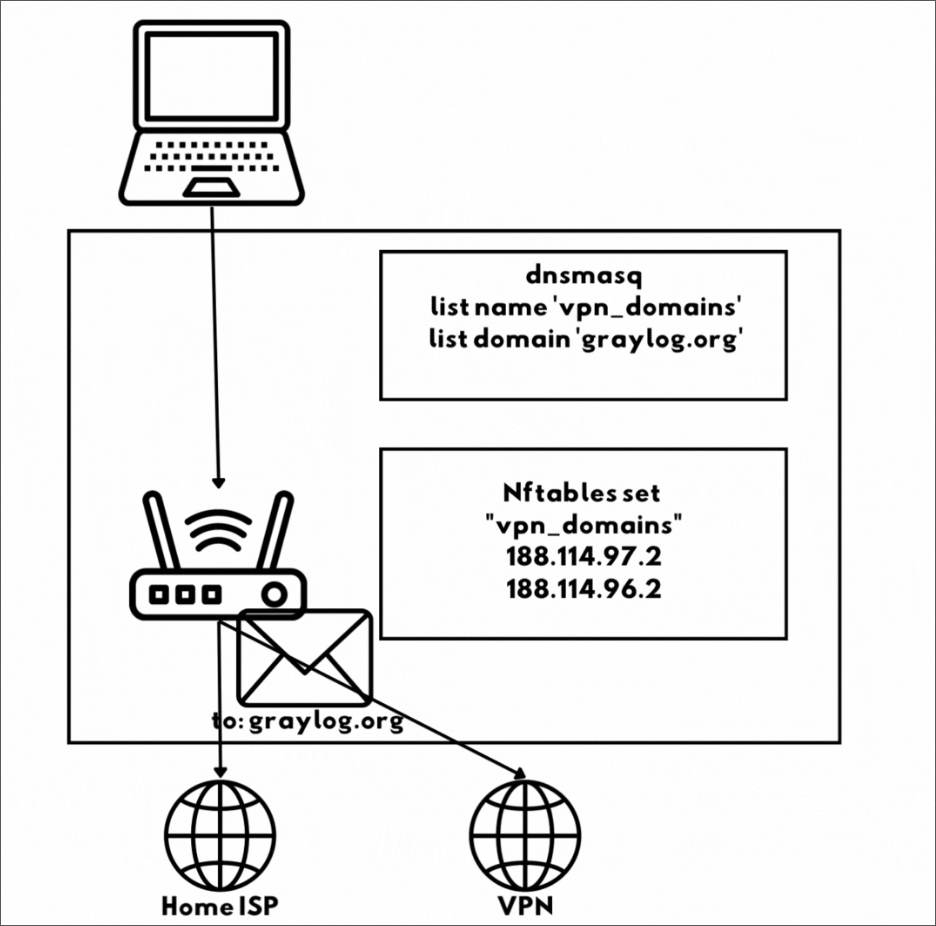
\includegraphics[scale=0.5]{inc/routing.png}
  \caption{Маршрутизация трафика}
  \label{fig:fig01}
\end{figure}
